\documentclass{scrartcl}

\usepackage{amssymb}
\usepackage{amsmath}
\usepackage{tikz}
\usetikzlibrary{decorations.pathreplacing}	%for brackets

%Das, M. \& N’Diaye, P. (2013). ``Chronicle of a Decline Foretold: Has China Reached the Lewis Turning Point?'' IMF Working Paper. Retrieved from http://www.imf.org/external/pubs/ft/wp/2013/wp1326.pdf

\begin{document}
	
	%\begin{figure}
	%	\centering
	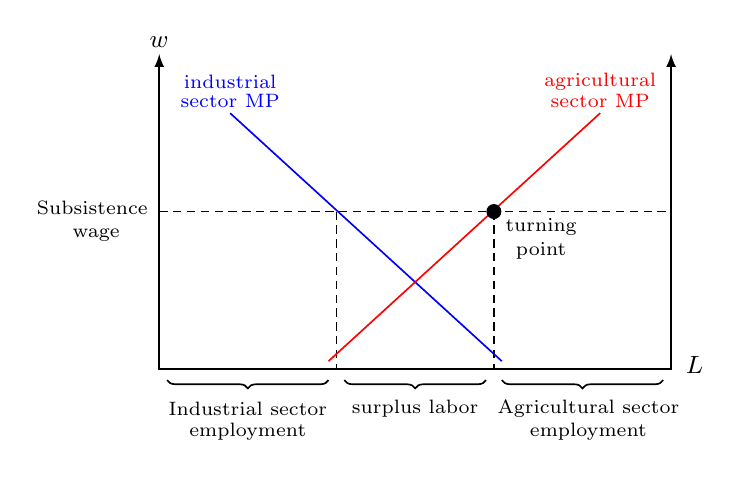
\begin{tikzpicture}
	%lines
	\draw[<->,>=latex,semithick] (0,4)--(0,0)--(6.5,0)--(6.5,4); %axis
	\draw[semithick,densely dashed] (0,2)--(6.5,2);		%subsistence
	\draw[semithick,densely dashed] (2.25,2)--(2.25,0);	%vertical, left
	\draw[semithick,densely dashed] (4.25,2)--(4.25,0);	%vertical, right
	\draw[semithick,blue] (0.9,3.25)--(4.35,0.1);		%industrial MP
	\draw[semithick,red]  (5.6,3.25)--(2.15,0.1);		%agri MP
	\filldraw (4.25,2) circle (2.5pt);					%turning point
	
	%upper labels
	\node at (0,4.15)  	 {\small $w$};	%wages
	\node at (6.8,0.05)  {\small $L$};	%labor force
	\node at (-.85,2.05) {\scriptsize Subsistence};
	\node at (-0.8,1.7)  {\scriptsize wage};
	\node at (4.85,1.8)  {\scriptsize turning};
	\node at (4.85,1.5)  {\scriptsize point};
	\node at (0.9,3.65)  {\textcolor{blue}{\scriptsize industrial}};
	\node at (0.9,3.40)  {\textcolor{blue}{\scriptsize sector MP}};
	\node at (5.6,3.65)  {\textcolor{red}{\scriptsize agricultural}};
	\node at (5.6,3.40)  {\textcolor{red}{\scriptsize sector MP}};
	
	%lower labels
	\draw[decorate,decoration={brace,amplitude=3pt},yshift=-4pt,semithick] (2.15,0)--(0.1,0);
	\draw[decorate,decoration={brace,amplitude=3pt},yshift=-4pt,semithick] (4.15,0)--(2.35,0);
	\draw[decorate,decoration={brace,amplitude=3pt},yshift=-4pt,semithick] (6.4,0)--(4.35,0);
	\node at (1.125,-0.5) {\scriptsize Industrial sector};
	\node at (1.125,-0.8) {\scriptsize employment};
	\node at (3.250,-0.5) {\scriptsize surplus labor};
	\node at (5.450,-0.5) {\scriptsize Agricultural sector};
	\node at (5.450,-0.8) {\scriptsize employment};
	\end{tikzpicture}
	%	\caption{The Lewis dual-sector model}
	%\end{figure}
	
\end{document}